\documentclass{report}
\usepackage[T1]{fontenc} % Fontes T1
\usepackage[utf8]{inputenc} % Input UTF8
\usepackage[backend=biber, style=ieee]{biblatex} % para usar bibliografia
\usepackage{csquotes}
\usepackage[portuguese]{babel} %Usar língua portuguesa
\usepackage{blindtext} % Gerar texto automaticamente
\usepackage[printonlyused]{acronym}
\usepackage{hyperref} % para autoref
\usepackage{graphicx}
\usepackage{listings}
\usepackage{xcolor}
\usepackage{graphicx}
\usepackage{caption}
\lstset{
    frame=tb, % draw a frame at the top and bottom of the code block
    tabsize=4, % tab space width
    showstringspaces=false, % don't mark spaces in strings
    numbers=left, % display line numbers on the left
    commentstyle=\color{green}, % comment color
    keywordstyle=\color{blue}, % keyword color
    stringstyle=\color{red} % string color
}

\bibliography{bibliografia}

\begin{document}
%%
% Definições
%
\def\titulo{Reconhecimento de Imagens}
\def\data{15 de junho de 2019}
\def\autores{Diogo Amaral,Guilherme Pereira,Luís Costa}
\def\autorescontactos{(93228) diogomra7@ua.pt, (93134) guilherme.pereira@ua.pt,(92996) joselcosta@ua.pt}
\def\versao{1.0}
\def\departamento{Departamento de Electrónica, Telecomunicações e Informática}
\def\empresa{Universidade de Aveiro}
\def\logotipo{ua.pdf}
%
%%%%%% CAPA %%%%%%
%
\begin{titlepage}

\begin{center}
%
\vspace*{50mm}
%
{\Huge \titulo}\\ 
%
\vspace{10mm}
%
{\Large \empresa}\\
%
\vspace{10mm}
%
{\LARGE \autores}\\ 
%
\vspace{30mm}
%
\begin{figure}[h]
\center
\includegraphics{\logotipo}
\end{figure}
%
\vspace{30mm}
\end{center}
%
\begin{flushright}
\versao
\end{flushright}
\end{titlepage}

%%  Página de Título %%
\title{%
{\Huge\textbf{\titulo}}\\
{\Large \departamento\\ \empresa}
}
%
\author{%
    \autores \\
    \autorescontactos
}
%
\date{\data}
%
\maketitle

\pagenumbering{roman}

%%%%%% RESUMO %%%%%%
\begin{abstract}
Hoje em dia, é um aspeto bastante óbvio a utilização de novas tecnologia em todas as atividades, e com isto, muitas áreas científicas têm aumentado em termos de informação e eficácia no seu determinado objetivo e função.
 
Com isto surge a ciência referente ao reconhecimento e classificação de imagens. O nosso projeto tem como objetivo criar um sistema em que seja possível dar \textit{upload} a imagens, pesquisar objetos, mostrar a lista de objetos(por imagem ou por nome) da nossa base de dados.

Para a resolução deste projeto foi utilizado algumas tecnologias já prefeitas, pois alguns conceitos só vão ser abordados nas futuras unidades curriculares. Para além da utilização destas funcionalidades foi desenvolvida uma\textit{Interface Web} que tem como finalidade ser a ligação entre todo o sistema. Foi também elaborado um ficheiro \textit{Python} que funciona como o "cérebro"  do sistema e apresenta diversos métodos.

Estes ficheiros e funcionalidades são melhores descritos no decorrer do relatório.
\end{abstract}

\tableofcontents
% \listoftables     % descomentar se necessário
% \listoffigures    % descomentar se necessário


%%%%%%%%%%%%%%%%%%%%%%%%%%%%%%%
\clearpage
\pagenumbering{arabic}

%%%%%%%%%%%%%%%%%%%%%%%%%%%%%%%%
\chapter{Introdução}
\label{chap.introducao}
Este relatório está dividido em 5 principais partes. A primeira é relativa a este \autoref{chap.introducao}, a introdução, fora esta componente existe o \autoref{chap.Objetivos} em que é descrita todo o projeto detalhadamente, desde as páginas \ac{html}, \ac{css}, \ac{js} até ao ficheiro \textit{Python}.

No \autoref{chap.Bónus} é apresentada a nossa ideia, para assim obter o bónus no nosso projeto.
No \autoref{chap.Testes efetuados} é descrito alguns testes feitos para assim verificar a correção das funções. No penúltimo capítulo, o \autoref{chap.Resultados} são analisados alguns resultados obtidos.

Para finalizar no \autoref{chap.Conclusao} é exposta uma pequena conclusão acerca deste trabalho e posteriormente as contribuições dos autores.

\chapter{Objetivos}
\label{chap.Objetivos}
\section{Interface Web}
Tal como foi explicitado anteriormente, a \textit{Interface Web} tem a função de interligar todas as funções do sistema, sendo esta dividida em 5 páginas(descritas separadamente de seguida). 

Para a realização destas páginas foi utilizado \ac{html} para criar a estrutura das páginas, \ac{css} para que o aspeto das páginas ficasse mais apelativo e dinâmico para o utilizador e \ac{js} para conciliação com o ficheiro em \textit{Python}.

\subsection{Listagem dos Objetos(por nome)}
Uma das páginas mostra a listagem dos objetos guardados na base de dados, sendos estes já detetados ou imagens introduzidas no sistema.
\newline
\begin{center}
   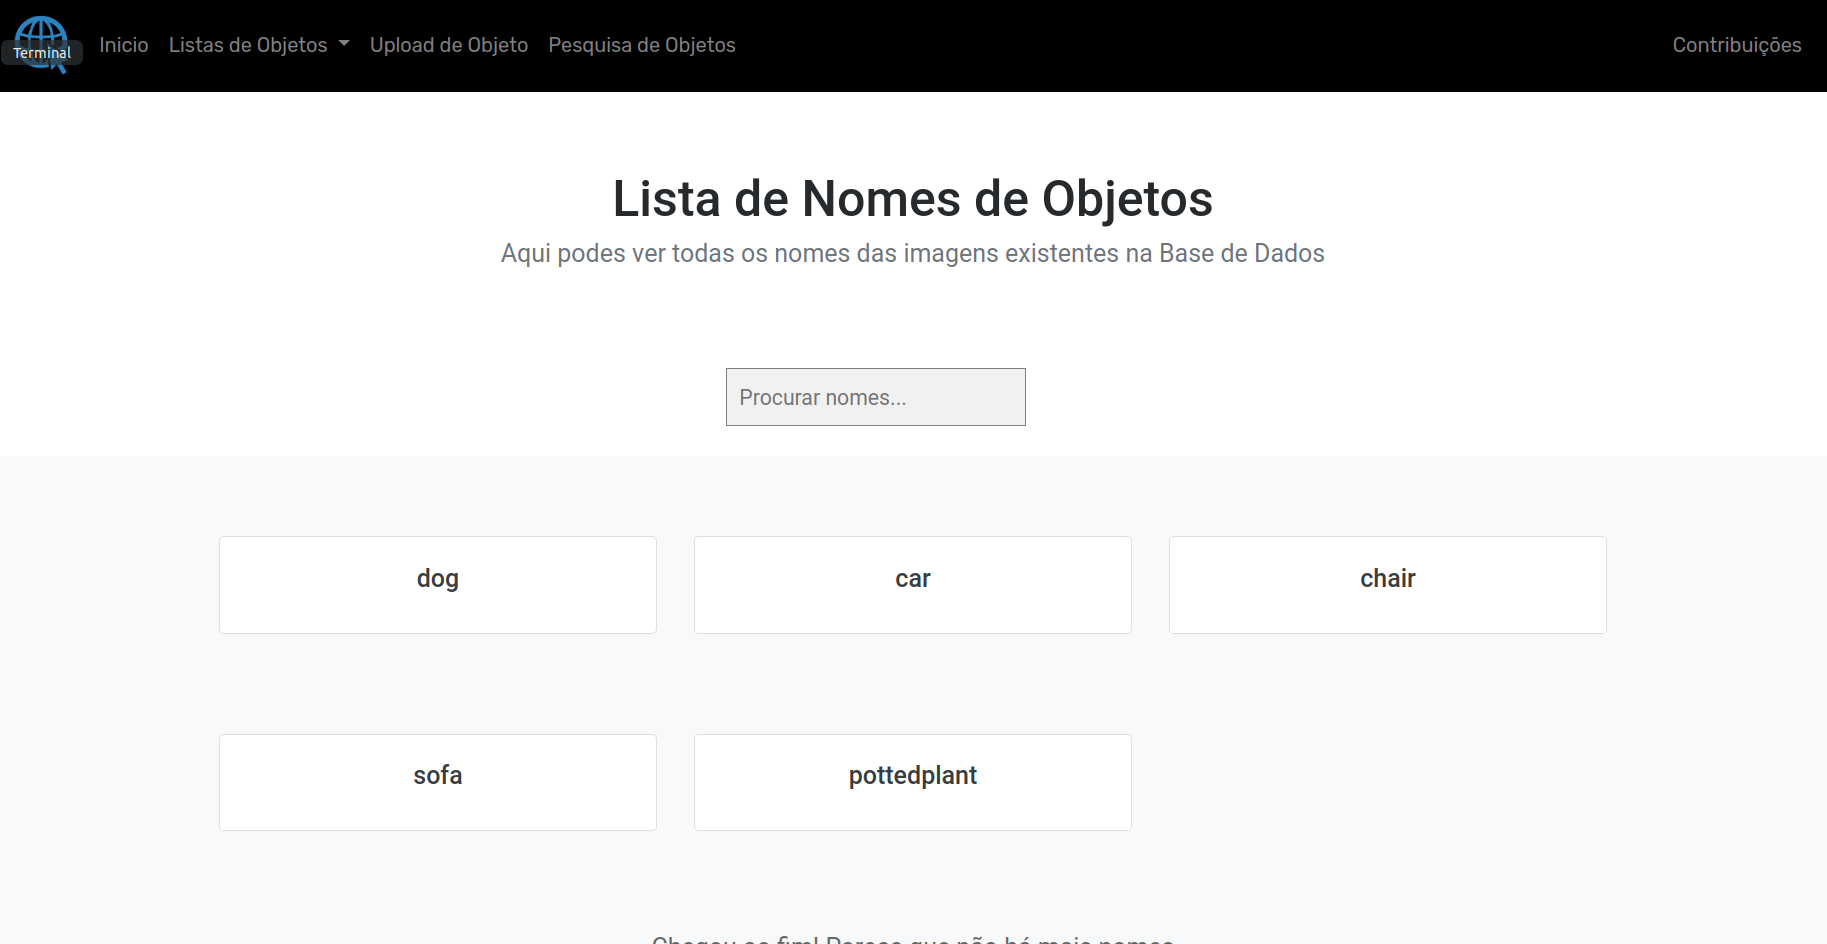
\includegraphics[scale=0.2]{listaObj.png}
   \captionof{figure}{Demonstração do site para listar objetos por nome}
\end{center}

\subsection{Listagem dos Objetos(por imagem)}
Esta página mostra a listagem dos objetos guardados na base de dados, mas neste caso, lista por imagem e não pelo nome(como o anterior).
\newline
\begin{center}
   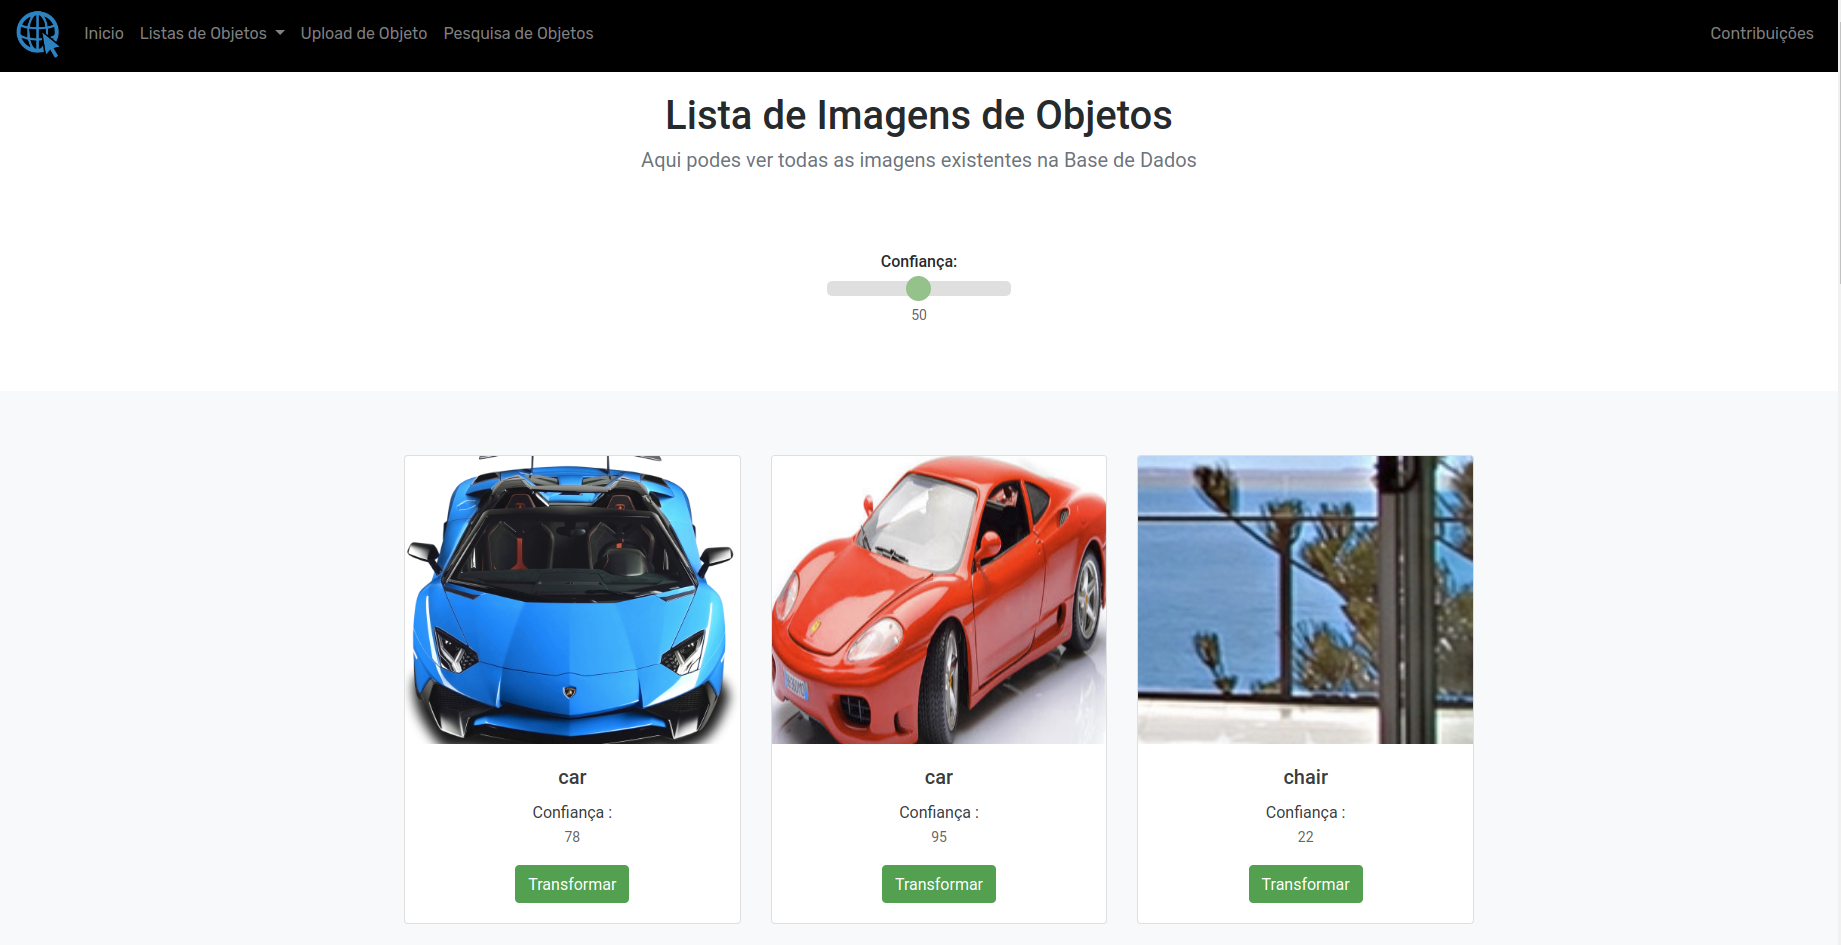
\includegraphics[scale=0.2]{listaImagem.png}
   \captionof{figure}{Demonstração do site para listar objetos por imagem}
\end{center}

\subsection{Upload de imagens}
Esta página é bastante importante, pois oferece a possibilidade de o utilizador dar \textit{upload} a uma imagem para a base de dados do sistema.

\begin{center}
   
\includegraphics[scale=0.2]{upload.png}
   \captionof{figure}{Upload de uma imagem}
\end{center}

\subsection{Pesquisa de imagens}
Esta penúltima página permite ao utilizador a pesquisa de um objeto de acordo com a cor e o seu tipo. Por exemplo, "red car", o sistema vai procurar imagens com grandes quantidades da cor vermelha, e do tipo descrito e vai mostra-las.

\begin{center}
   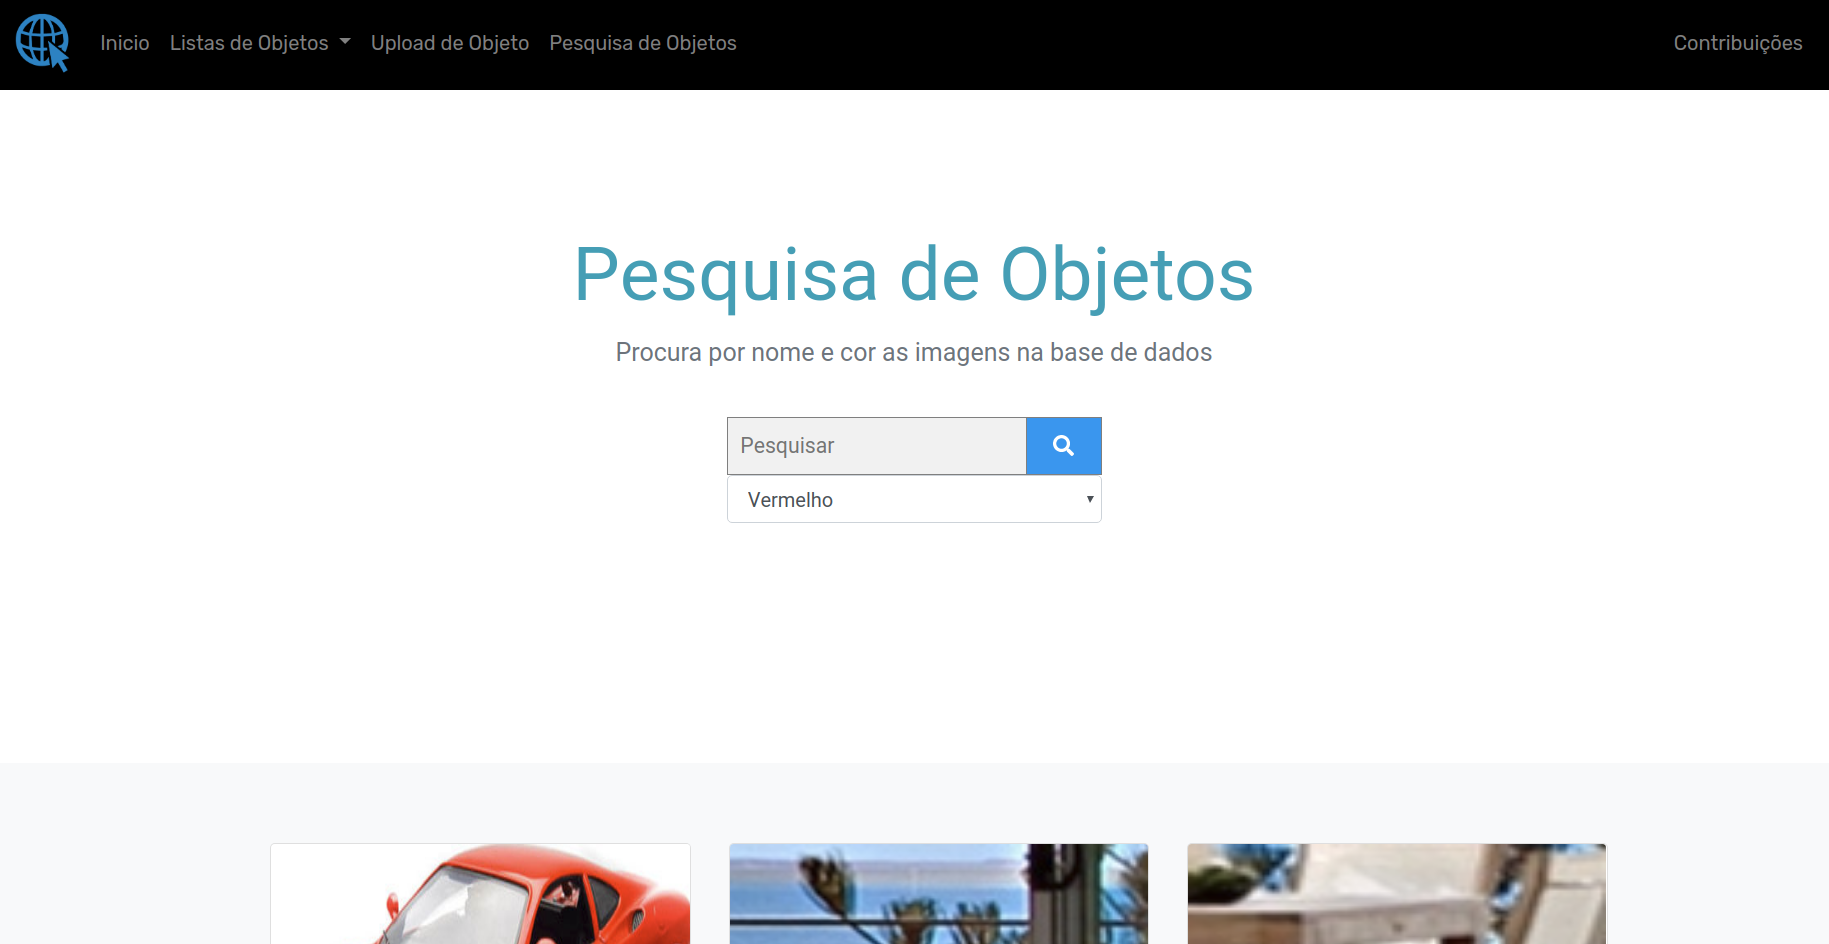
\includegraphics[scale=0.2]{pesq.png}
   \captionof{figure}{Upload de uma imagem}
\end{center}

\section{Aplicação Web}


\subsection{/list?type=names:}
Esta função devolve um \ac{json} contendo todos os objetos que forram detetados pelo sistema.

\begin{lstlisting}[language=Python, caption={getAllNames}] 
def getAllNames():
    result = db.execute("Select Nome From Base WHERE IsObject = 'true' ")
    rows = [rows[0] for rows in result.fetchall()]
    data = {} 
    rows = list(dict.fromkeys(rows))
    data['Nomes'] = rows
    return json.dumps(data, indent=4, sort_keys=True)
\end{lstlisting}


\subsection{/list?type=detected:}
Esta função retorna uma lista com pequenas imagens recortadas com objetos extraídos.

\begin{lstlisting}[language=Python, caption={getDetectedObjects}] 
def getDetectedObjects():
  names = db.execute("Select Nome From Base WHERE IsObject = 'true'")
  allNamesRows = [rows[0] for rows in names.fetchall()]
  singleNamerows = list(dict.fromkeys(allNamesRows))
  data = {}
  for singleNames in singleNamerows: 
    data[singleNames] = [] 
    ids = db.execute("Select ObjId From Base WHERE Nome = ?", (singleNames,)) 
    for id in ids:
      imgHash = db.execute("Select ImgId From Base WHERE ObjId = ?", (id)) 
      acc = db.execute("Select Acc From Base WHERE ObjId = ?", (id))
      objHash = db.execute("Select ObjId From Base WHERE ObjId = ?", (id)) 
      idDic = {} 
      idDic["image"] = [rows[0] for rows in objHash.fetchall()][0] 
      idDic["confidence"] = [rows[0] for rows in acc.fetchall()][0]
      idDic["original"] = [row[0] for row in imgHash.fetchall()][0] 
      data[singleNames].append(idDic)
return json.dumps(data, indent=4, sort_keys=True)
\end{lstlisting}


\subsection{/list?type=detected\&name=NAME:}
Esta função retorna uma lista com pequenas imagens recortadas com objetos específicos. Este método é igual ao getDetectedObjects mas com a diferença de confirmar o nome do objeto.
\begin{lstlisting}[language=Python, caption={getDetectedObjectsByName}] 
def getDetectedObjectsByName(name):
(...)
if singleNames == name :
\end{lstlisting}

\subsection{/list?type=detected\&name=NAME\&color=COLOR:}
Esta função retorna uma lista com pequenas imagens recortadas com objetos específicos. Este método é igual ao getDetectedObjects mas com a diferença de confirmar a cor do objeto.

\begin{lstlisting}[language=Python, caption={getDetectedObjectsByColor}] 
def getDetectedObjectsByColor(name, color):
\end{lstlisting}

\subsection{/put:}
Esta função permite adicionar uma nova imagem:
\begin{lstlisting}[language=Python, caption={addToDatabase}] 
def upload(self, ufile):
  upload_file = os.path.normpath(os.path.join("img/", ufile.filename))
  if(len(ufile.filename) != 0) :
    file = open(upload_file, 'wb')
    while True:
      data = ufile.file.read(8192)
      if not data:
        break
      file.write(data)
    msg = allImageProcessing("img/" + (...))
  
\end{lstlisting}


\subsection{/get?id=IDENTIFIER:}
Esta função permite, com o \textit{Id} de uma imagem, obter uma certa imagem:

\begin{lstlisting}[language=Python, caption={getById}] 
def getById(id): 
  try:
    img = db.execute("Select objPath From Base WHERE ObjId = ?", (id,))
    result = [row[0] for row in img.fetchall()][0]
    return json.dumps(result, indent=4, sort_keys=True)
\end{lstlisting}


\section{Persistência}
Esta parte do projeto tem como função guardar e aceder às informações numa base de dados. Para a produção da base de dados foi utilizado o \textit{sqlite3}. Estes métodos vão ser utilizados pela \textit{Aplicação Web} para obter as cores, a identificação dos objetos, registar imagens, etc...

\section{Processador de imagens}
Esta função é dada pelos professores da unidade curricular, e tem como objetivo processar uma imagem para o sistema.
\begin{lstlisting}[language=Python, caption={getImageInfo}] 
def getImageInfo(path):
  session = requests.Session()
  URL="http://image-dnn-sgh-jpbarraca.ws.atnog.av.it.pt/process"
  with open(path, 'rb') as f:
    file = {'img': f.read()}
    r = session.post(url=URL, files=file, data=dict(thr=0.01))
    if r.status_code == 200:
      imgValues = r.json()
    else:
      imgValues = "null"

    return imgValues
\end{lstlisting}
\chapter{Bónus}
\label{chap.Bónus}
Com a finalidade de o sistema oferecer mais funcionalidades ao utilizador, implementámos uma função para que seja permitido alterar uma imagem, usando filtro, neste caso cinzento ou sépia.

Ao clicar na \textit{Listagem de Imagens de Objetos} irá aparecer o botão \textit{Transformar}(tal como é demostrado no ponto 2.1.2) que nos levará para outra página onde é possível escolher entre os dois filtros.

\begin{center}
   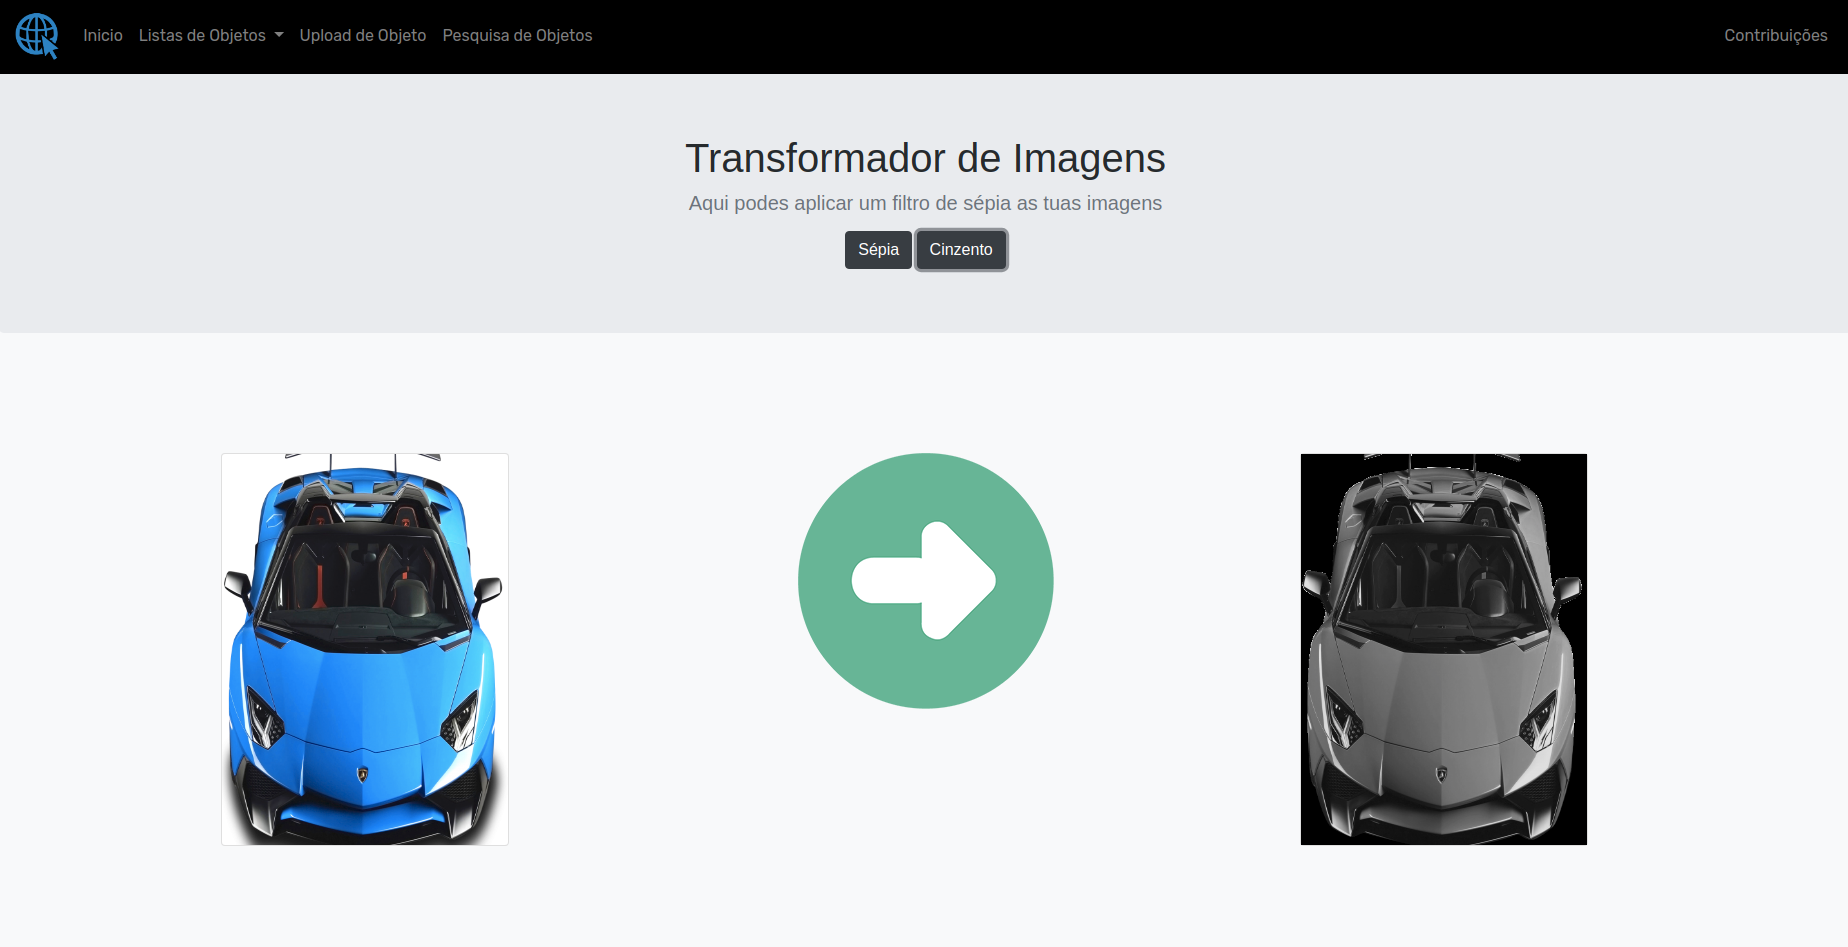
\includegraphics[scale=0.2]{filtro.png}
   \captionof{figure}{Exemplo, usando o filtro cizento}
\end{center}
  
\chapter{Testes efetuados}
\label{chap.Testes efetuados}
Um dos testes efetuados, para verificar o bom funcionamento do sistema, é por exemplo, introduzir uma imagem e verificar as funções do sistema.


Introduzir a imagem:
\begin{center}
   
\includegraphics[scale=0.2]{up.png}
   \captionof{figure}{Upload}
\end{center}

Se pesquisarmos "car" e escolhermos a cor "azul", irá aparecer, tal como suposto, a imagem introduzida. Também nas listas vai acontecer tudo como o previsto, assim demonstrando um bom funcionamento do sistema (comprovado nas seguintes imagens).
\begin{center}  
  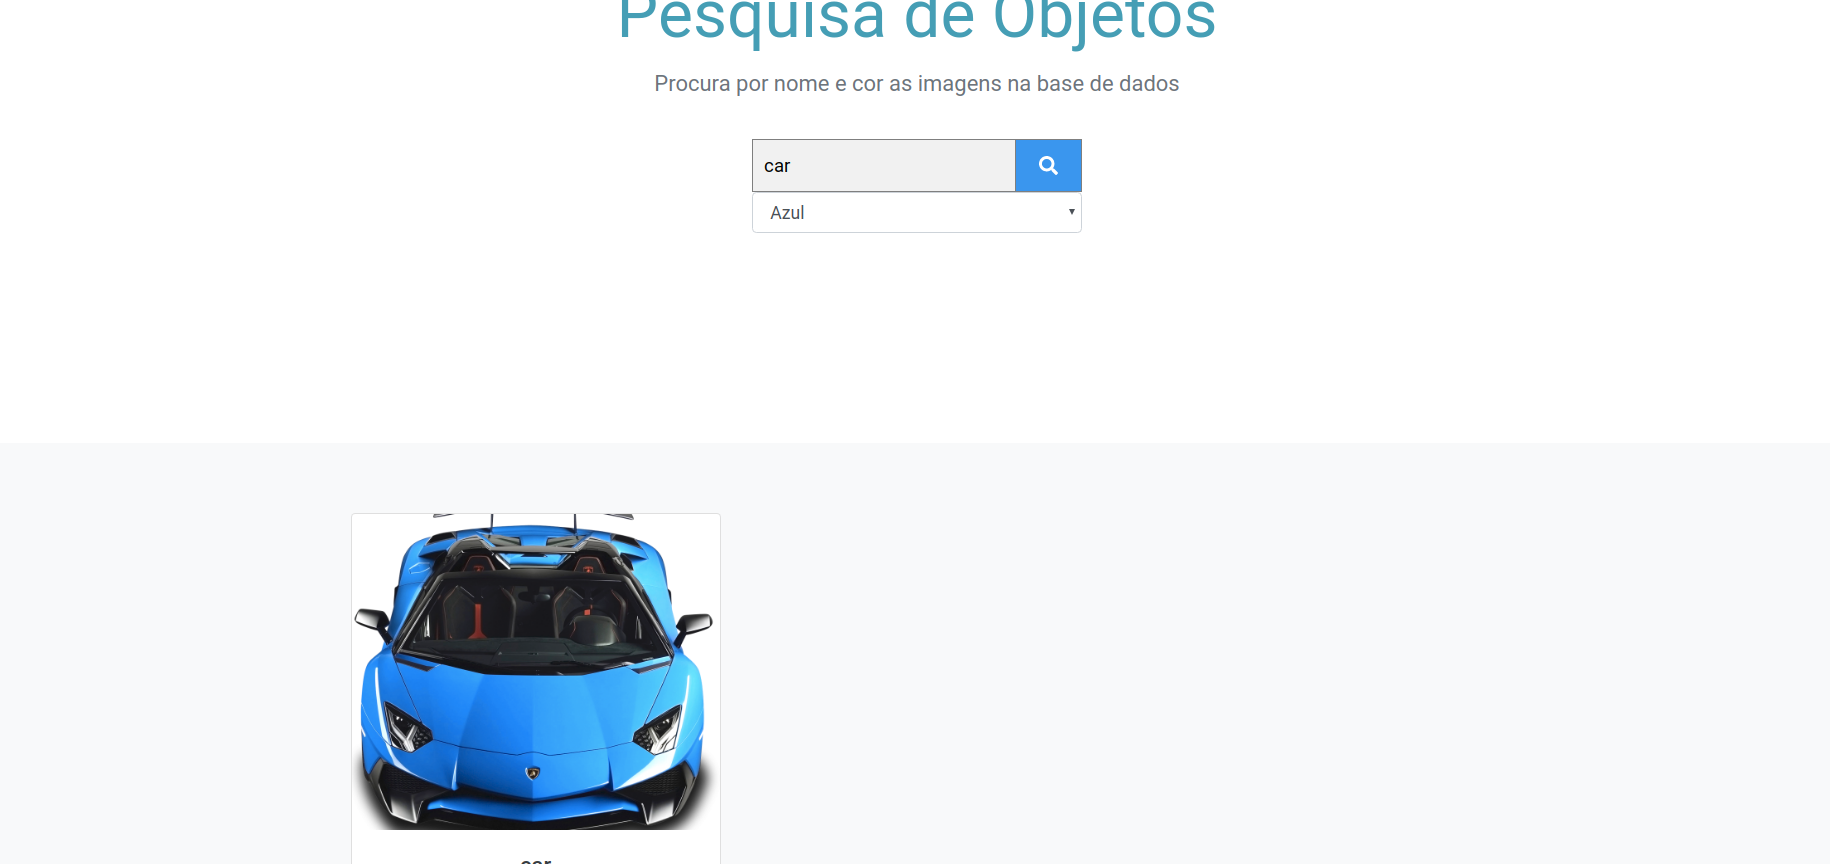
\includegraphics[scale=0.2]{lista.png}
   \captionof{figure}{Demonstração de pesquisa por cor e objeto}
\end{center}

\begin{center}  
  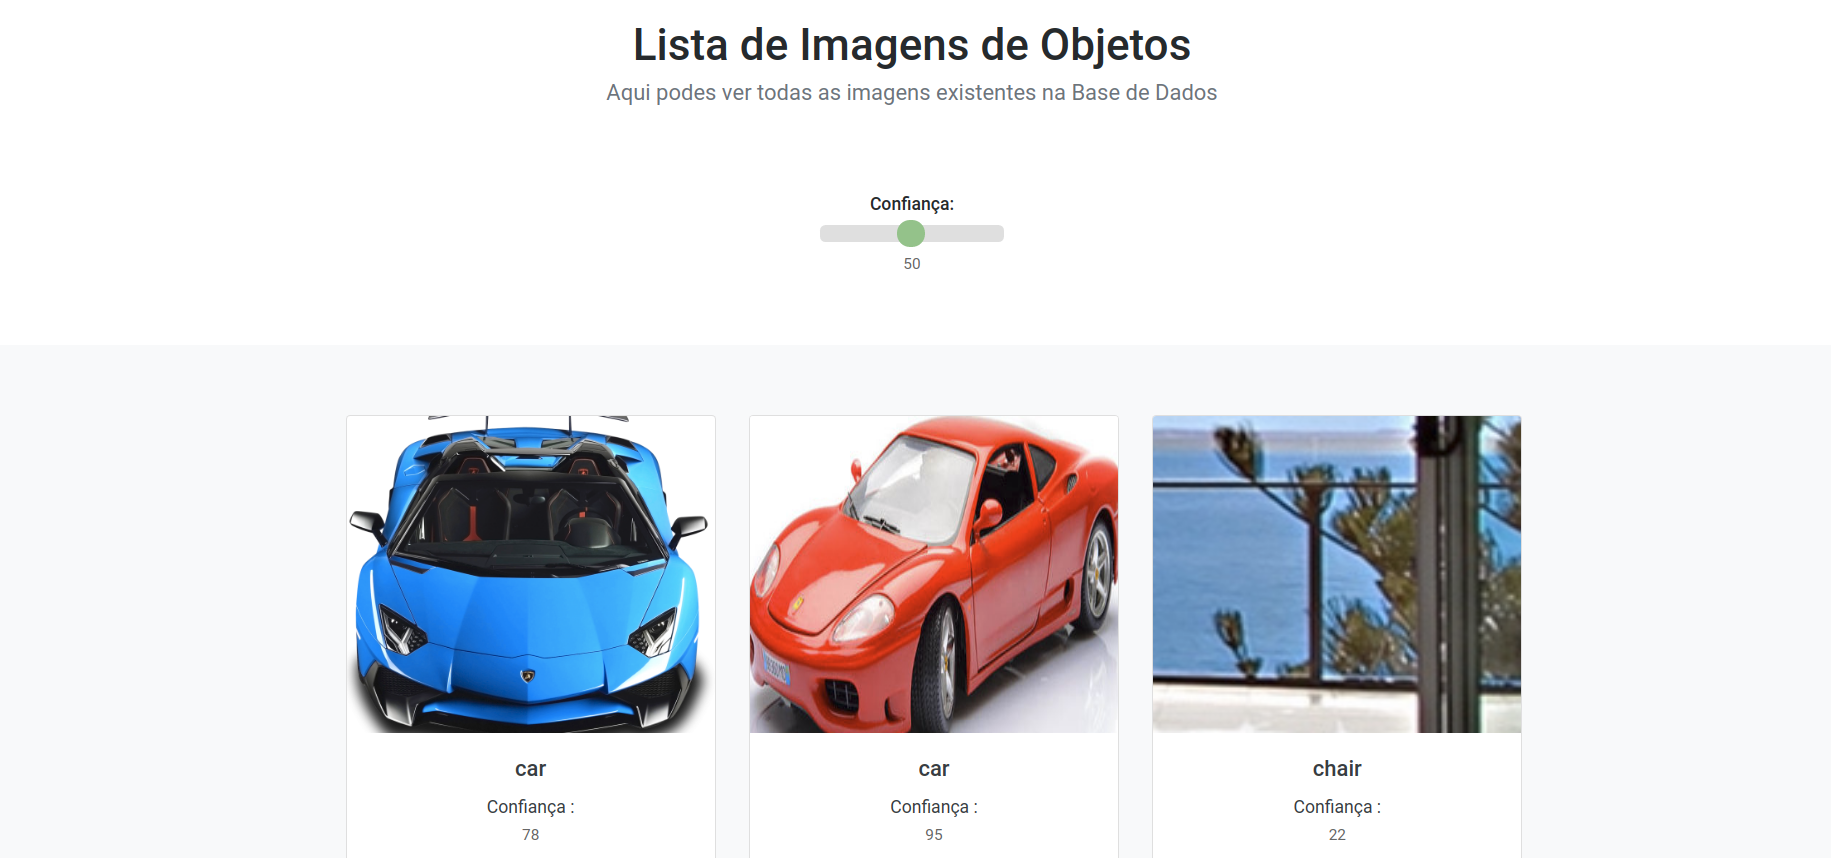
\includegraphics[scale=0.2]{pesquisa.png}
   \captionof{figure}{Demonstração da listagem da base de dados}
\end{center}


\chapter{Resultados}
\label{chap.Resultados}
Com base no \autoref{chap.Testes efetuados} podemos analisar o funcionamento do sistema. Ao ser introduzido a imagem na base de dados, e posteriormente com a listagem desta, podemos verificar que a imagem foi introduzido com sucesso. 

A pesquisa por cor e objeto, do mesmo modo que a listagem, ajuda-nos a perceber que o sistema está a correr como o suposto pois para selecionar apenas as imagens com o objeto escolhido e a cor escolhida é necessário verificar os itens na base de dados e em seguida mostrar apenas aqueles que correspondem aos requisitos do utilizador.

Os restantos serviços a dispor do utilizador, são mais uma vez, uma confirmação do funcionamento correto do sistema dado que fazem tudo o que é suposto.

\chapter{Conclusões}
\label{chap.Conclusao}

Neste trabalho concluímos que é bastante importante a classificação e determinação de objetos para diversas áreas cientificas, sendo cada vez mais, por exemplo, com o avanço da inteligência artificial. Desta forma, o nosso projeto pode abrir novos horizontes para algumas aplicações e sistemas.

Como este projeto é o projeto final, tivemos uma especial atenção em realizar tudo com as maior competências e correção possível para assim o projeto ficar na sua melhor versão, e achamos que foi conseguido com clareza.

\chapter*{Contribuições dos autores}

Para a produção deste projeto final, todos os membros do grupo esforçaram-se para que este trabalho fosse concluído com o maior sucesso. O Guilherme Pereira na realização do site e do ficheiro python, o Luís Costas mais focado na base de dados e no ficheiro python e o Diogo Amaral na produção do site e do relatório final. 

Assim atribuindo a mesma percentagem a cada membro do grupo, 33\% ao Guilherme Pereria, 33\% ao Diogo Amaral e 33\% ao Luís Costa.

CodeUA: \url{http://code.ua.pt//projects/labi2019-p2-g4}

Xcoa: \url{https://xcoa.av.it.pt/labi2019-p2-g4/index.html}
%%%%%%%%%%%%%%%%%%%%%%%%%%%%%%%%%
\chapter*{Acrónimos}
\begin{acronym}
\acro{html}[HTML]{HyperText Markup Language}
\acro{css}[CSS]{Cascading Style Sheets}
\acro{js}[JS]{JavaScript}
\acro{json}[JSON]{JavaScript Object Notation}
\end{acronym}


%%%%%%%%%%%%%%%%%%%%%%%%%%%%%%%%%
\printbibliography

\end{document}